%laden der Präambel mit Latexbefehlen/-klassen
% !TeX encoding = UTF-8

%Dokumentklasse, Spracheinstellung, Schriften
\documentclass[a0paper,portrait]{baposter}
\usepackage[english]{babel}
\usepackage[utf8]{inputenc}
\usepackage{arev}
%\usepackage[T1]{fontenc}

%Mathe, Symbole, Einheitendarstellung, Chemie
\usepackage{amsmath}
\usepackage{amsxtra}
\usepackage{eurosym}
\usepackage{siunitx}  
\sisetup{locale=US}
\usepackage[version=4]{mhchem}

%Typographie
\usepackage[auto]{microtype}

%Einbindung von Bildern, Tabellen, pdf-Seiten, Quellcode
\usepackage{booktabs}
\usepackage{multirow}
\usepackage{paralist}
\usepackage{graphicx}

%Darstellung der Literaturangaben
\usepackage[
backend=biber,
style=science,
citestyle=numeric-comp,
sorting=none,
maxbibnames=1,
firstinits=true
]{biblatex}

\bibliography{refs}
\setlength\bibitemsep{2.5pt}

%Definition der Farben
\definecolor{standardfontcolor}{RGB}{0,0,0} 
\definecolor{bordercol}{RGB}{255,255,255}
% \definecolor{bordercol}{RGB}{29,29,29}
\definecolor{headercol1}{RGB}{255,255,255}
\definecolor{headercol2}{RGB}{166,25,46}
% \definecolor{headercol2}{RGB}{113,113,113}
\definecolor{headerfontcol}{RGB}{0,0,0}
\definecolor{boxcolor}{RGB}{255,255,255}

\begin{document}

%	\background{
%		\begin{tikzpicture}[remember picture,overlay]%
%			\draw (current page.north west)+(-2em,2em) node[anchor=north west]
%				{\includegraphics[height=1.1\textheight]{bilder/logo/logo-gruppe-1.pdf}};
%		\end{tikzpicture}
%	}

	\color{standardfontcolor}

	\begin{poster}{
		grid=false,
		columns=6,
	%colspacing=length
		headerheight=0.075\textheight,
		eyecatcher=true,
		borderColor=bordercol,
		headerColorOne=headercol1,
		headerColorTwo=headercol2,
		headerFontColor=headerfontcol,
		boxColorOne=boxcolor,
		headershape=rectangle,
		headerfont=\sffamily\bfseries\Large,
		textborder=rectangle,
		headerborder=open,
		boxshade=plain,
		background=none
	% background=user
	}
	% logo left
	{
		
\includegraphics[height=2cm]{figs/logo/VirginiaScienceLover.png}\hspace{0.3cm}\vspace{-3cm}
		
\includegraphics[height=2cm]{figs/logo/jlab_logo}
	}
	% title and author
	{
		\textsf %Sans Serif
		{The Heavy Photon Search Experiment}
	}
	{
		\sf\vspace{0.5em}\\
		HPS Collaboration
	}
	% logo right
	{
		\hspace{2cm}
		
\includegraphics[height=3cm]{figs/logo/heavy_photon_logo.jpg}
	}

		\headerbox{What are Heavy Photons?}{name=intro,column=0,row=0,span=3}{
% \hspace{0.01\columnwidth}%
			\begin{minipage}{0.44\columnwidth}
				To understand what Heavy Photons are, we first need to understand what Dark Matter is.\\
				From cosmological observations (i.e. looking at the stars), we know that there must be more matter in our Universe than what we can see. One of these observations is that spiral galaxies rotate faster than we would expect them to based on the number of stars that make up the galaxy.\\
				If we assume that there is some sort of `invisible' matter in those galaxies in addition to the visible matter consisting of stars and alike, our theoretical predictions and actual observations match again.
			\end{minipage}
			\begin{minipage}{0.56\columnwidth}
				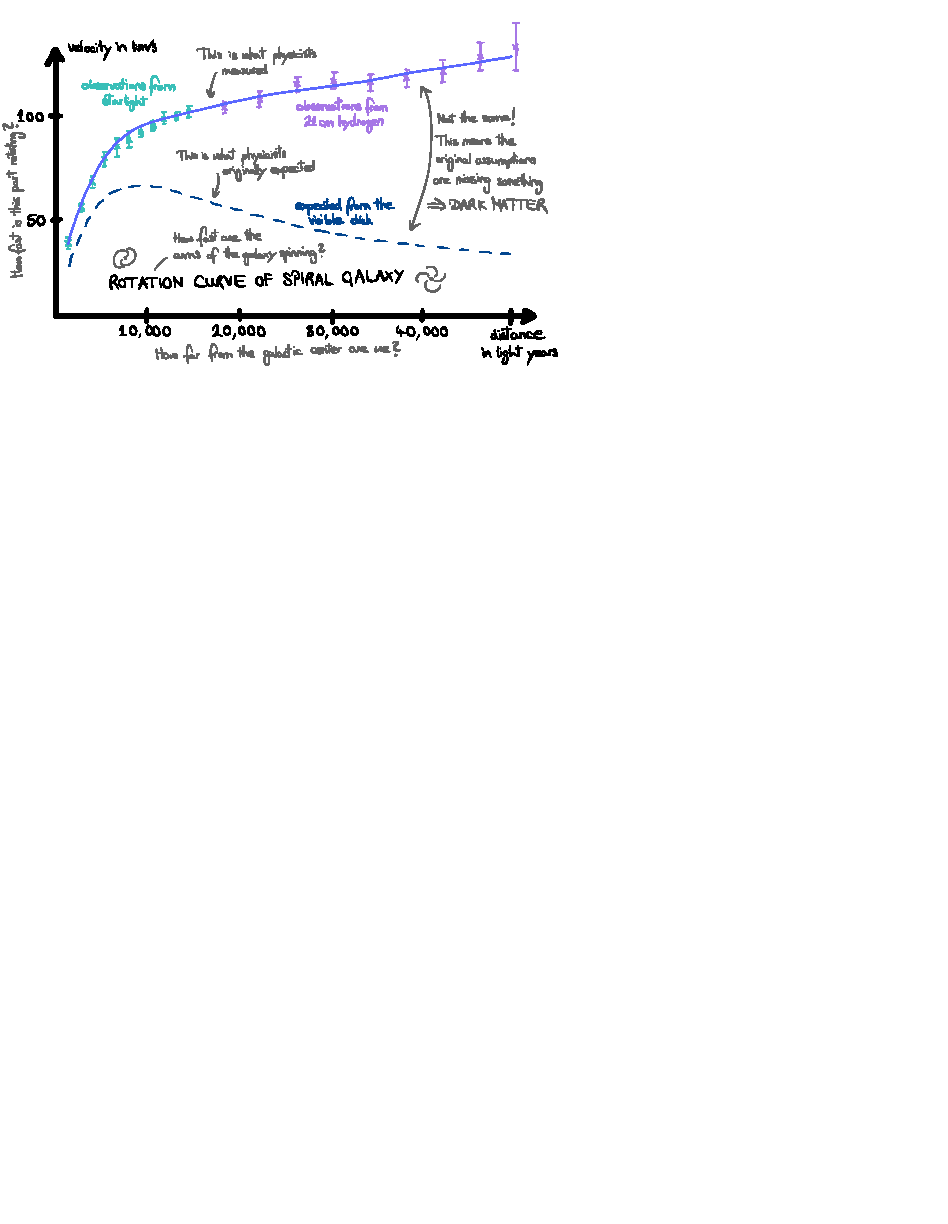
\includegraphics[width=\columnwidth]{figs/rotationCurve.pdf}
			\end{minipage}
			\begin{minipage}{0.44\columnwidth}
				\centering
				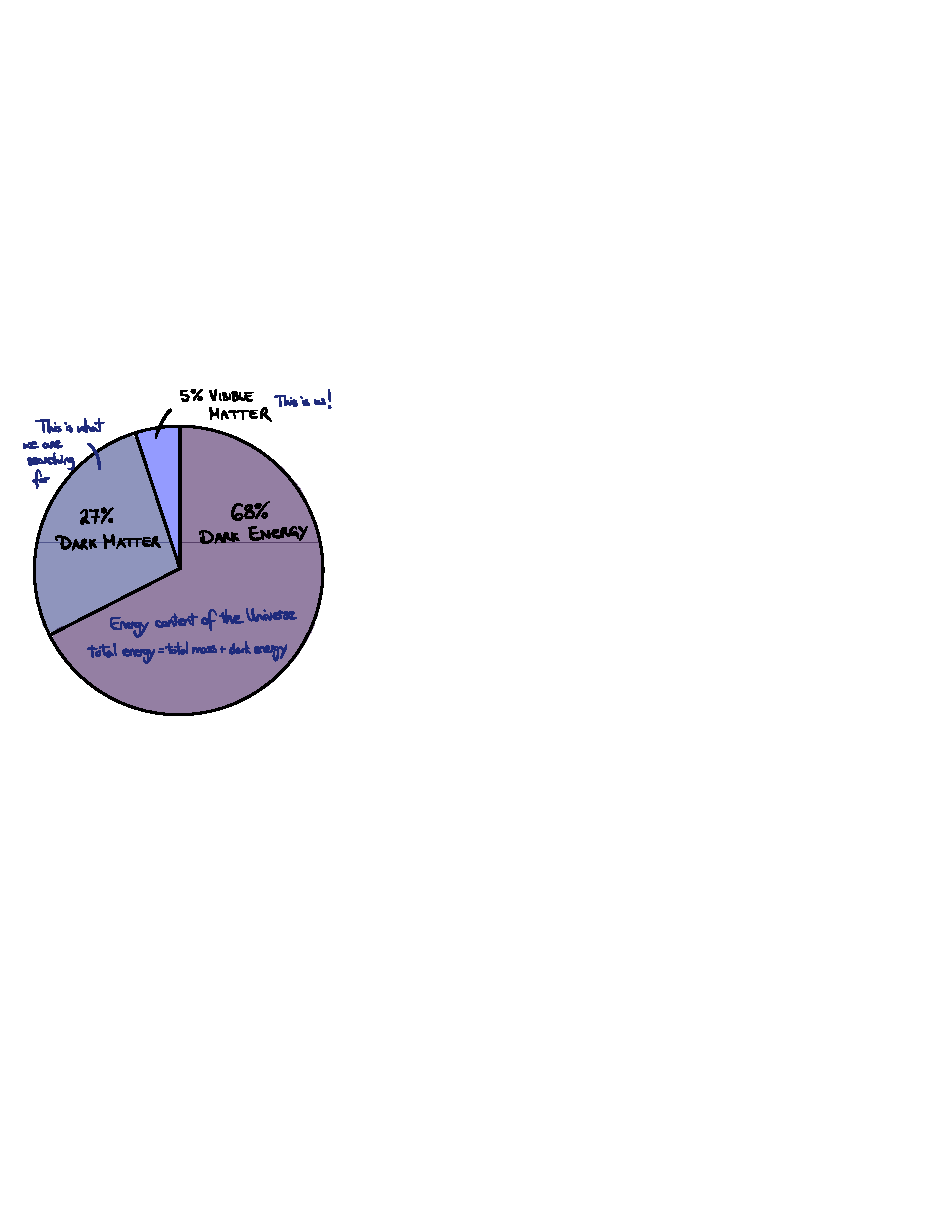
\includegraphics[width=0.7\columnwidth]{figs/pieUniverse.pdf}
			\end{minipage}
			\hspace{0.01\columnwidth}%
			\begin{minipage}{0.56\columnwidth}
				In fact, it turns out that we expect about 5 times more Dark Matter than regular matter in our Universe! But what is this mysterious Dark Matter? Currently, we only know that Dark Matter has mass and doesn't like to interact with regular matter.\\
				One theory about Dark Matter tells us that there could be a `Dark Sector'. You can imagine this Dark Sector as a universe existing parallel to ours with its own physical laws. In our theory of the Dark Sector, there is a `Heavy Photon' (sometimes `dark photon') that behaves so similarly to the real-world photon that it occasionally transforms into one. When this happens, the Heavy Photon can decay into an electron and a positron (the electron's anti-particle) which we can detect in our experiment.
			\end{minipage}
		}

		\headerbox{How are we searching for them?}{name=search,column=3,span=3}{
			\includegraphics[width=\columnwidth]{figs/HPS_detector_GeneralPublic.pdf}
%			{\color{white}i}
			\hspace{0.06\columnwidth}%
			\begin{minipage}{0.46\columnwidth}
				The Silicon Vertex Tracker (SVT) consists of multiple `Silicon Strip' sensors. Each time a particle passes through a sensor, it leaves behind some of its energy. Like this, we can measure where the particle passed through the sensor and connect the dots to find its path.
			\end{minipage}%
			\hspace{0.1\columnwidth}%
			\begin{minipage}{0.39\columnwidth}
				The Electromagnetic Calorimeter (ECAL) consists of 442 lead-tungstate crystals. In these crystals, the energy of particles gets converted to UV light. By measuring how much light is created we can determine the particle's energy.
			\end{minipage}
		}

		\headerbox{Did you know?}{name=funfacts,column=0,below=intro,span=2}{
			\begin{compactitem}
				\item Each module in the SVT must be very light (less than an ounce!) and thin, so particles don't slow down and scatter in random directions.
				\item The SVT strips have a width smaller than the diameter of a human hair. And there are many of them! About 25000 strips are each connected to an electronic channel.
				\item Best in class: High amounts of radiation can damage silicon detectors. Closer to the electron beam, the detector has to withstand more radiation. Our SVT is the first to be located so close (\SI{0.5}{mm}) to a high luminosity electron beam.
				\item The SVT operates in a high magnetic field which is about 4 times stronger than magnetic fields that can erase credit cards or damage pacemakers.
			\end{compactitem}
		}

		\headerbox{Who are we?}{name=institutions,column=0,below=funfacts,span=2}{
			Finding dark matter is a communal effort: professors, staff and project scientists, graduate and summer students from around the world work together to discover Heavy Photons.\\

			\begin{minipage}{0.55\columnwidth}
				\centering
				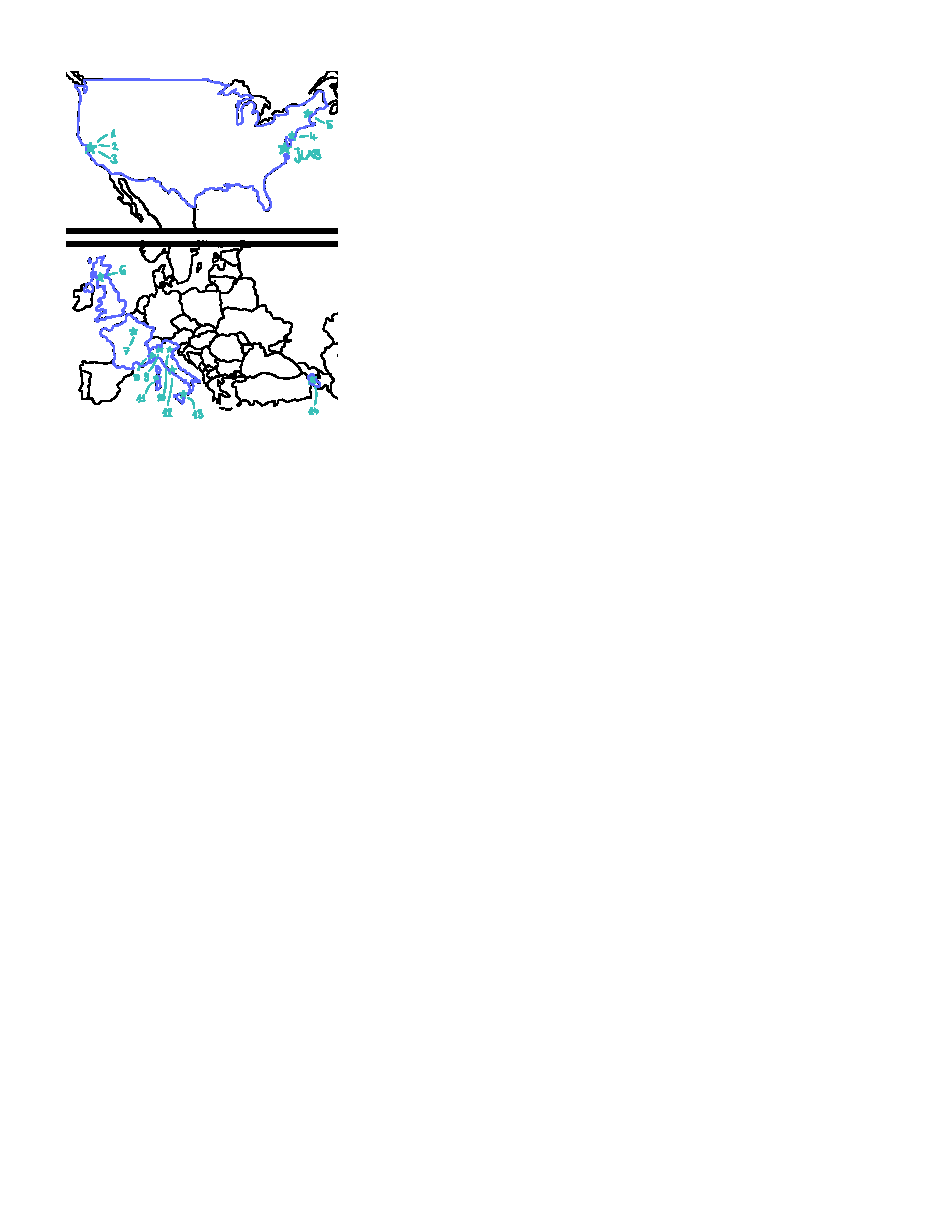
\includegraphics[width=0.9\columnwidth]{figs/collabMap.pdf}
			\end{minipage}%
			\begin{minipage}{0.45\columnwidth}
				\begin{compactitem}
					\item[1] SLAC
					\item[2] Stanford
					\item[3] University of California\\ Santa Cruz
					\item[4] Stony Brook
					\item[5] University of\\ New Hampshire
					\item[6] University of\\ Glasgow
					\item[7] Institut de Physique\\ Nucleaire d’Orsay
					\item[8]-- 13 INFN
					\item[14] Alikhanyan National\\ Science Laboratory
					\item[]
				\end{compactitem}
			\end{minipage}
		}


		\headerbox{Working on HPS}{name=work,column=2,below=intro,span=4}{
			\begin{minipage}{0.27\columnwidth}
				\centering
				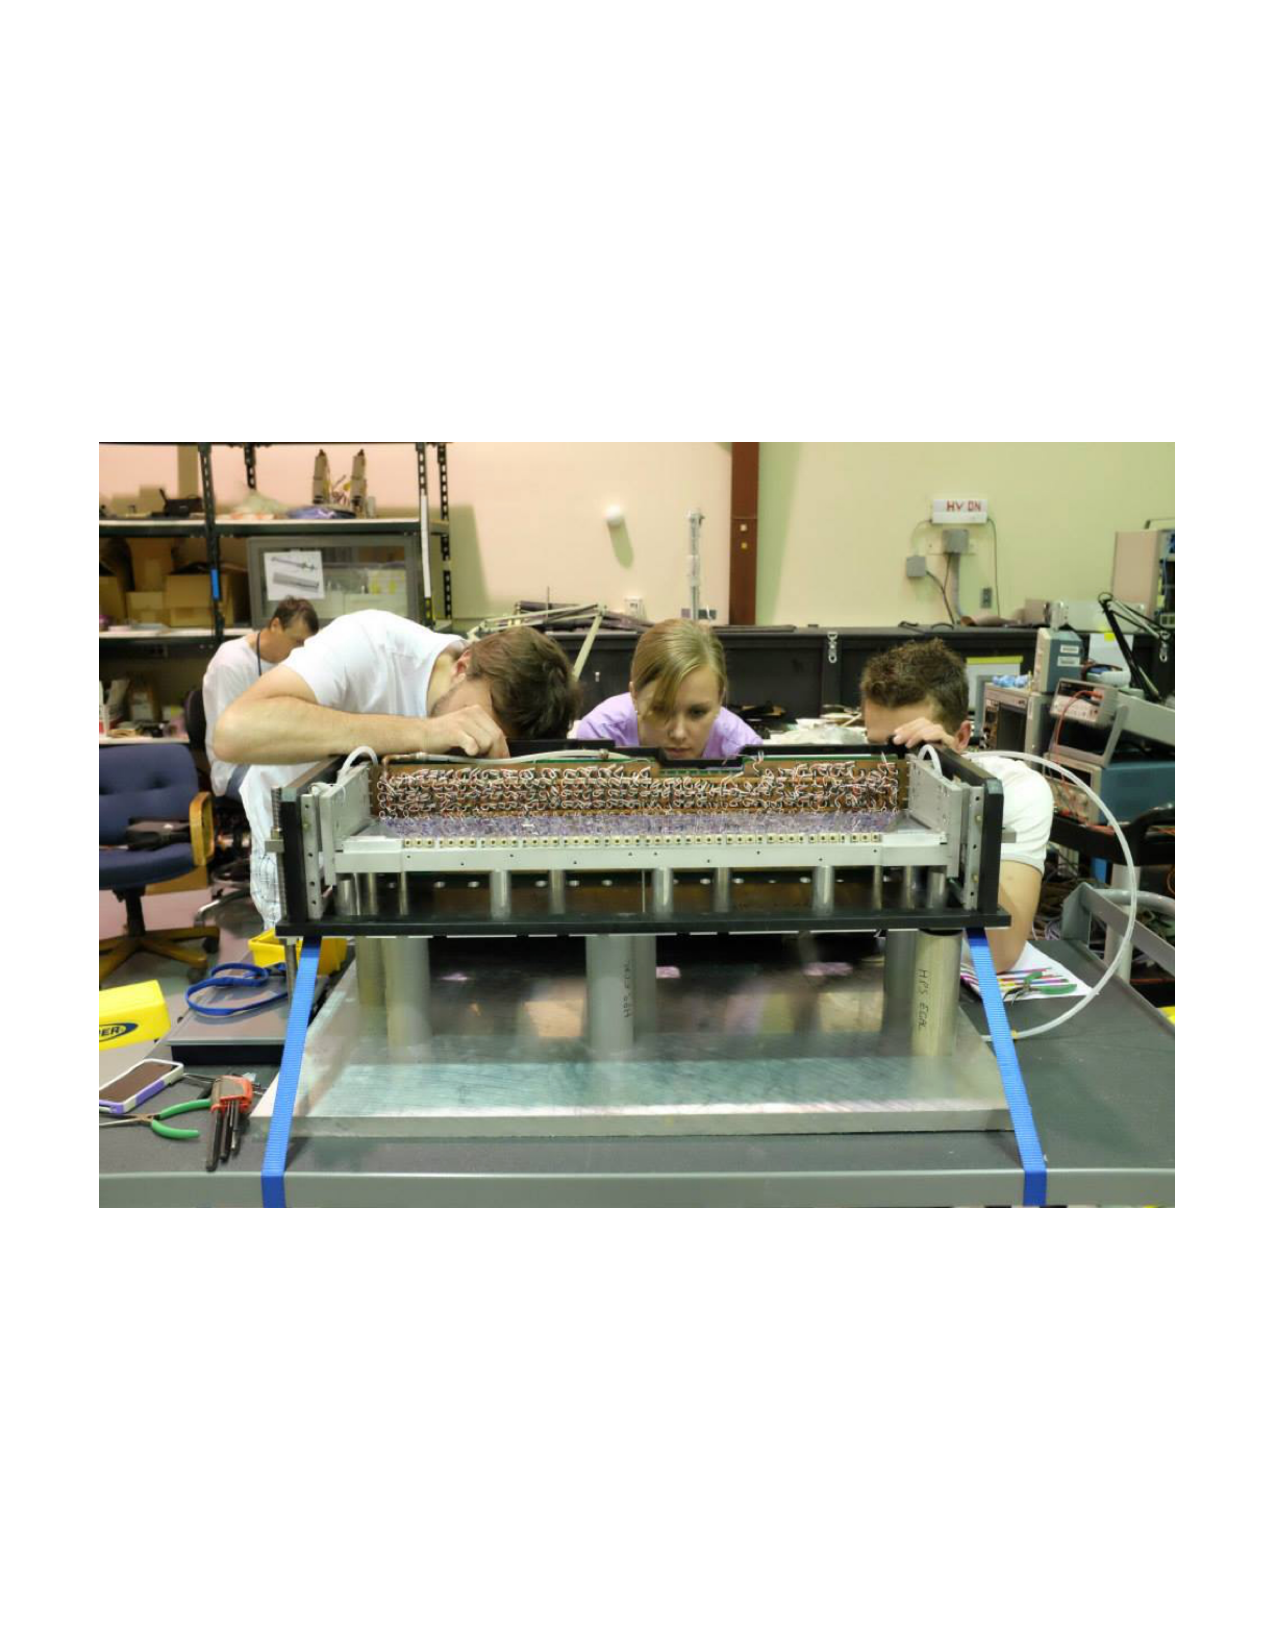
\includegraphics[width=\columnwidth]{figs/Calorimeter.pdf}
				ECAL assembly\\
				{\color{white} hhk\\}
				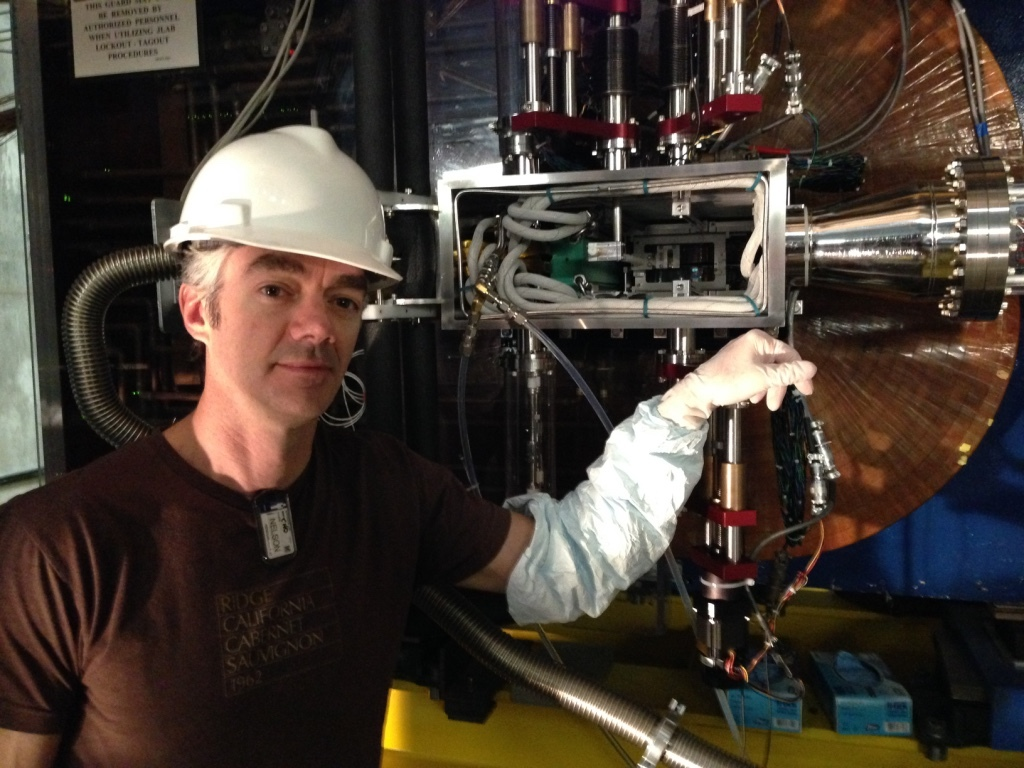
\includegraphics[width=\columnwidth]{figs/Tim_with_detector.jpeg}
				Our detector (human for scale)\\
				{\color{white} hhk\\}
				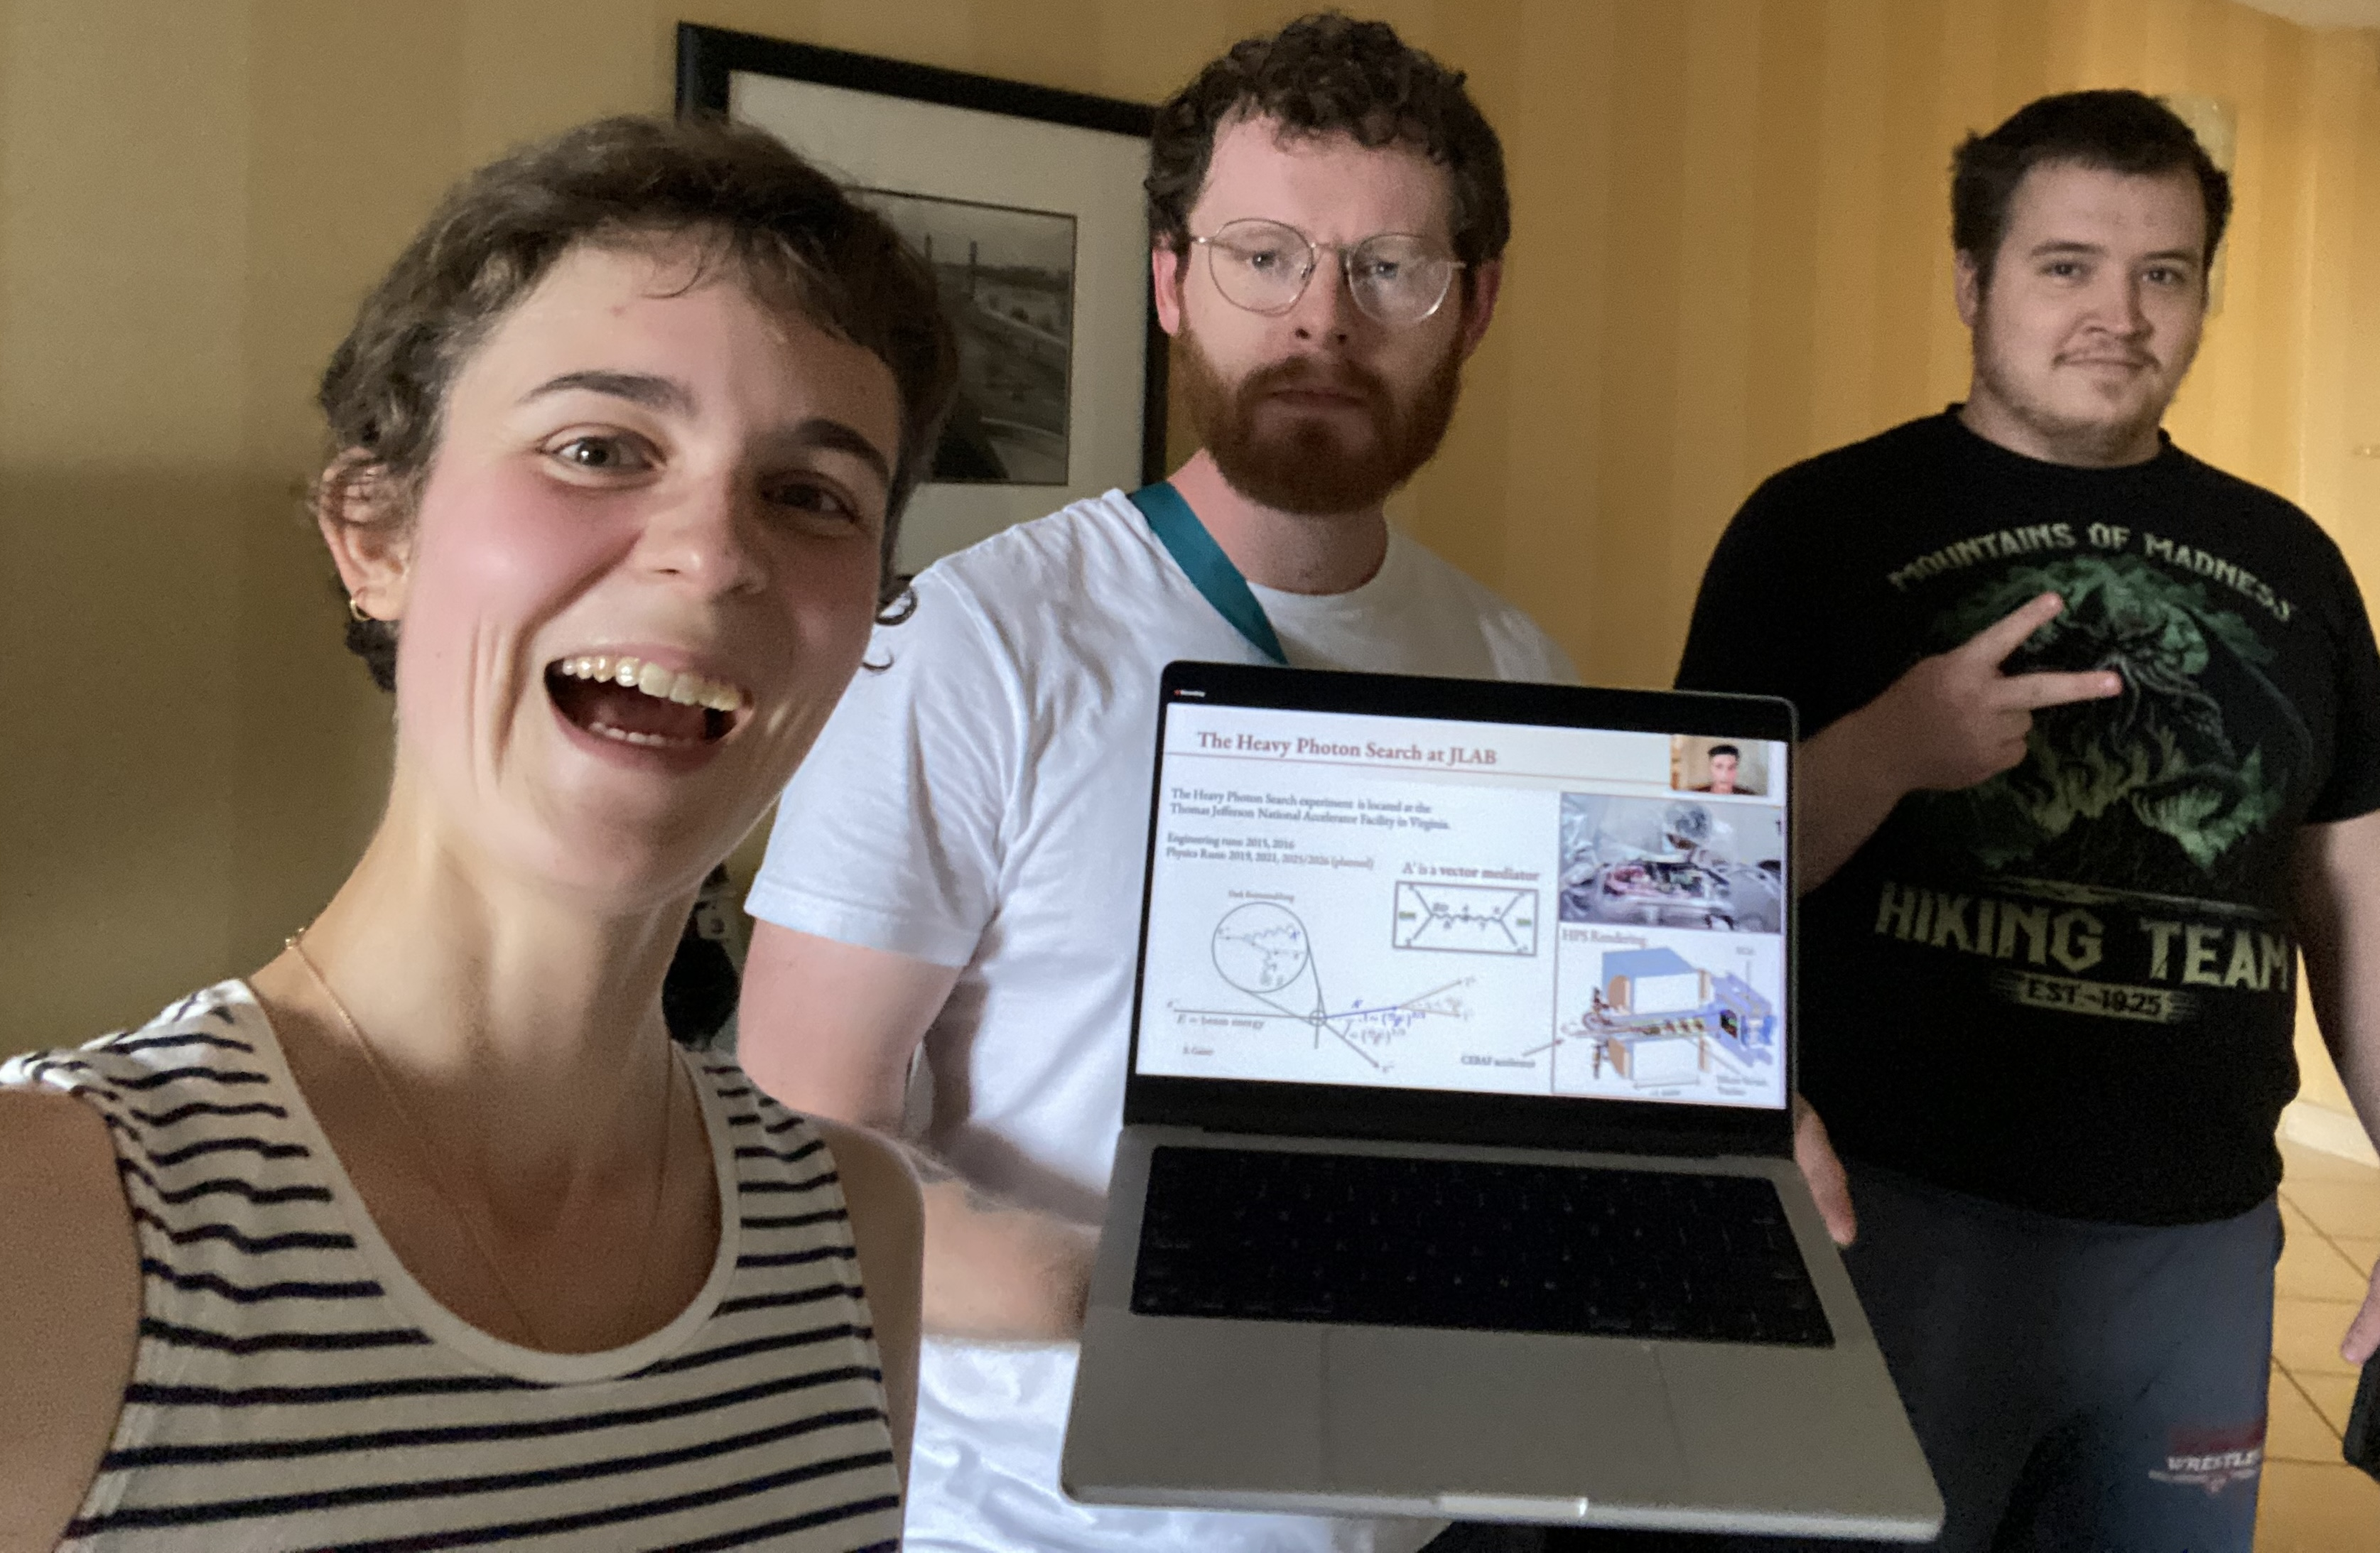
\includegraphics[width=\columnwidth]{figs/GradStudents.jpg}
				Grad students at the APS Meeting
			\end{minipage}%
			\hspace{0.01\columnwidth}%
			\begin{minipage}{0.43\columnwidth}
			{When running a particle physics experiment, there are many different things to do:
				\begin{compactitem}
					\item[]
					\item \textbf{Design and build the detector}: Starting in 2013, the HPS Collaboration came together to design and build the experimental setup that we are working with today.
					\item \textbf{Run the experiment}: Data is taken more or less non-stop in week-long periods called `runs'. During a run, we have to monitor our setup and fix it if necessary.
					\item \textbf{Data analysis}: Once the data is taken, we have to analyze it. We work on this with specialized software, some of which we programmed ourselves.
					\item \textbf{Presentation}: Last but not least, we are presenting our results in the form of scientific papers, talks at conferences, and posters like this one!
				\end{compactitem}
			}
			{\color{white} hhk}
			{\centering
			\includegraphics[width=\columnwidth]{figs/SVTassembly.pdf}
			Brain surgery? No, SVT construction.\\}
			\end{minipage}
			\hspace{0.01\columnwidth}%
			\begin{minipage}{0.27\columnwidth}
				\centering
				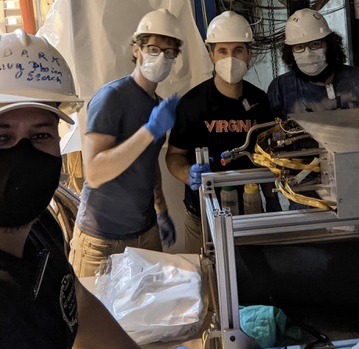
\includegraphics[width=\columnwidth]{figs/SVT_push.png}
				SVT installation\\
				{\color{white} hhk\\}
				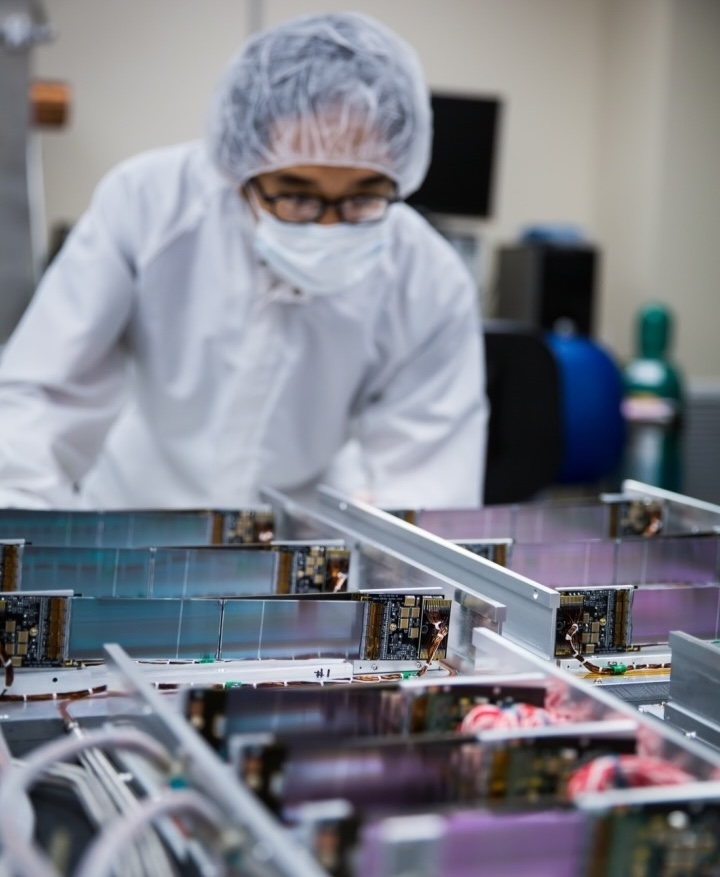
\includegraphics[width=\columnwidth]{figs/SVT_nice.jpeg}
				Building the SVT
			\end{minipage}%
		}


		\headerbox{HPS in action}{name=action,column=0,below=work,span=4}{
			\begin{minipage}{0.65\columnwidth}
				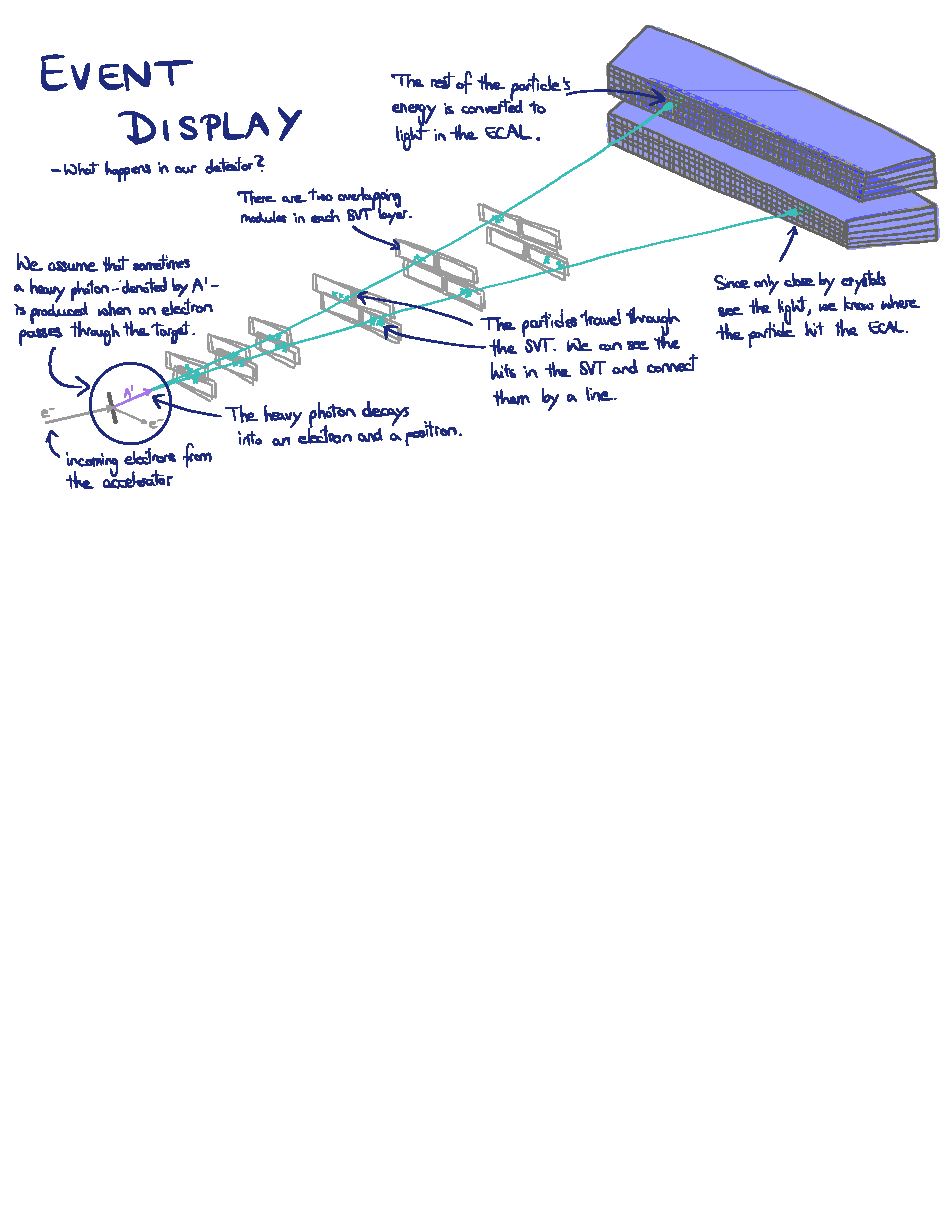
\includegraphics[width=\columnwidth]{figs/eventDisplay.pdf}
			\end{minipage}%
			\hspace{0.01\columnwidth}%
			\begin{minipage}{0.33\columnwidth}
				\textbf{What happens in the HPS detector when we run our experiment?}\\ A Heavy Photon (A', purple line) is created at the target and decays into an electron and a positron (blue lines) which travel through the detector. The SVT registers where each particle passes through its layers (blue marks). This is how we reconstruct the paths of the particles. When the electron and positron hit the ECAL, they generate small amounts of light (blue ellipses). The measured light tells us how much energy the particles have and where it hit the ECAL. Putting all this together, we have enough information to understand the physical process at the target.
			\end{minipage}
			\begin{minipage}{0.54\columnwidth}
				\textbf{Did we see a Heavy Photon or something else?} -- This is the central question of our analysis. From our theory, we predict the behavior of the Heavy Photon. When we see an event that matches our expectations, we call this a `signal'.\\
				It can be very tricky to distinguish between signal and background events. Thankfully, we know that we can describe our background by another theory called Quantum Electrodynamics (QED). This well-established theory tells us how many background events we expect. If the Heavy Photon exists, we will count more events at a certain energy, as illustrated in the top graphic on the right.\\
				Another method is to look at the common origin of the electron and positron tracks, the so-called vertex position. We expect that all background events originate from the target. The Heavy Photon events on the other hand can have a `displaced vertex' that lies behind the target as seen from the direction of the beam. This is illustrated in the lower panel on the right.
			\end{minipage}%
			\hspace{0.02\columnwidth}%
			\begin{minipage}{0.44\columnwidth}
				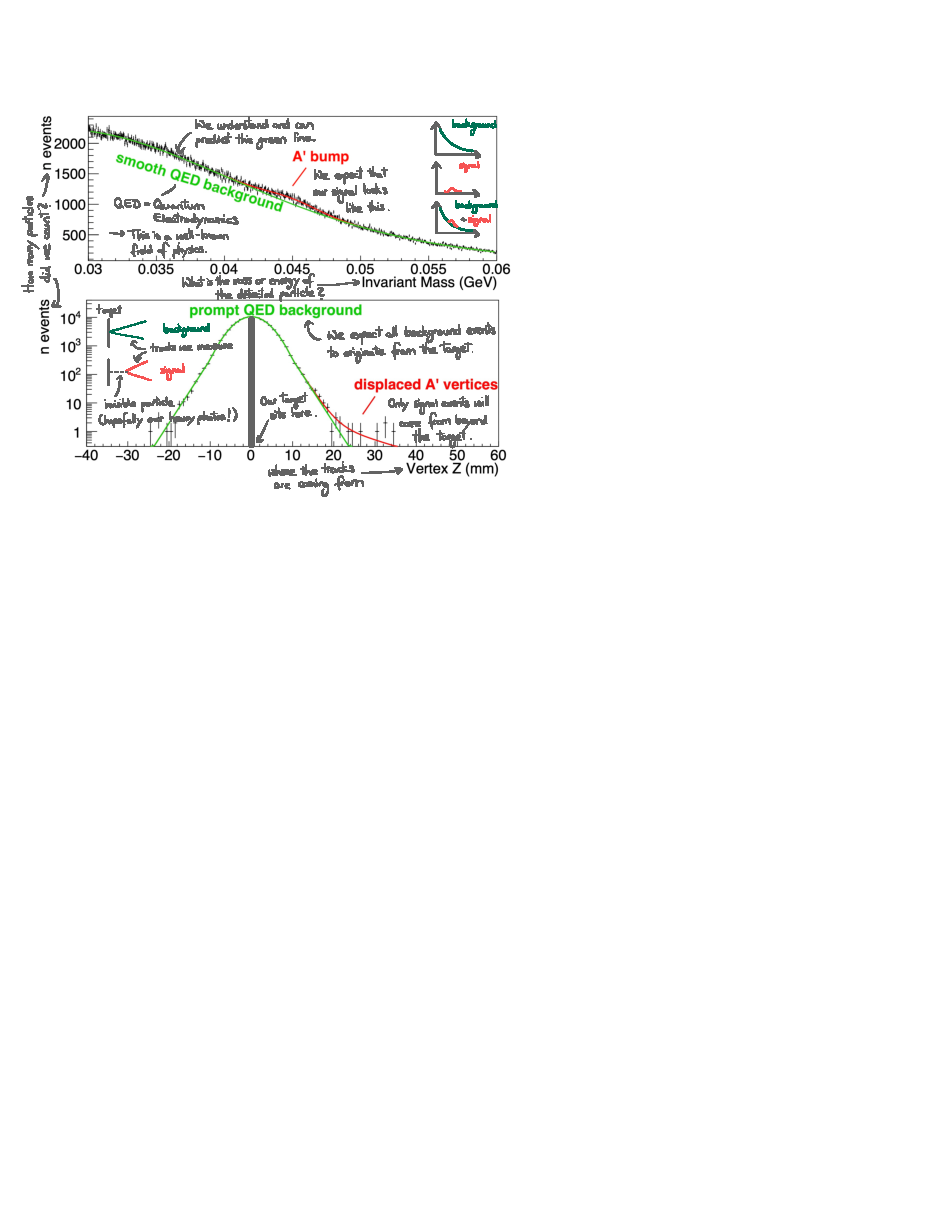
\includegraphics[width=\columnwidth]{figs/signalExplanation.pdf}
			\end{minipage}
		}

		\headerbox{Results}{name=results,column=4,below=work,span=2}{
			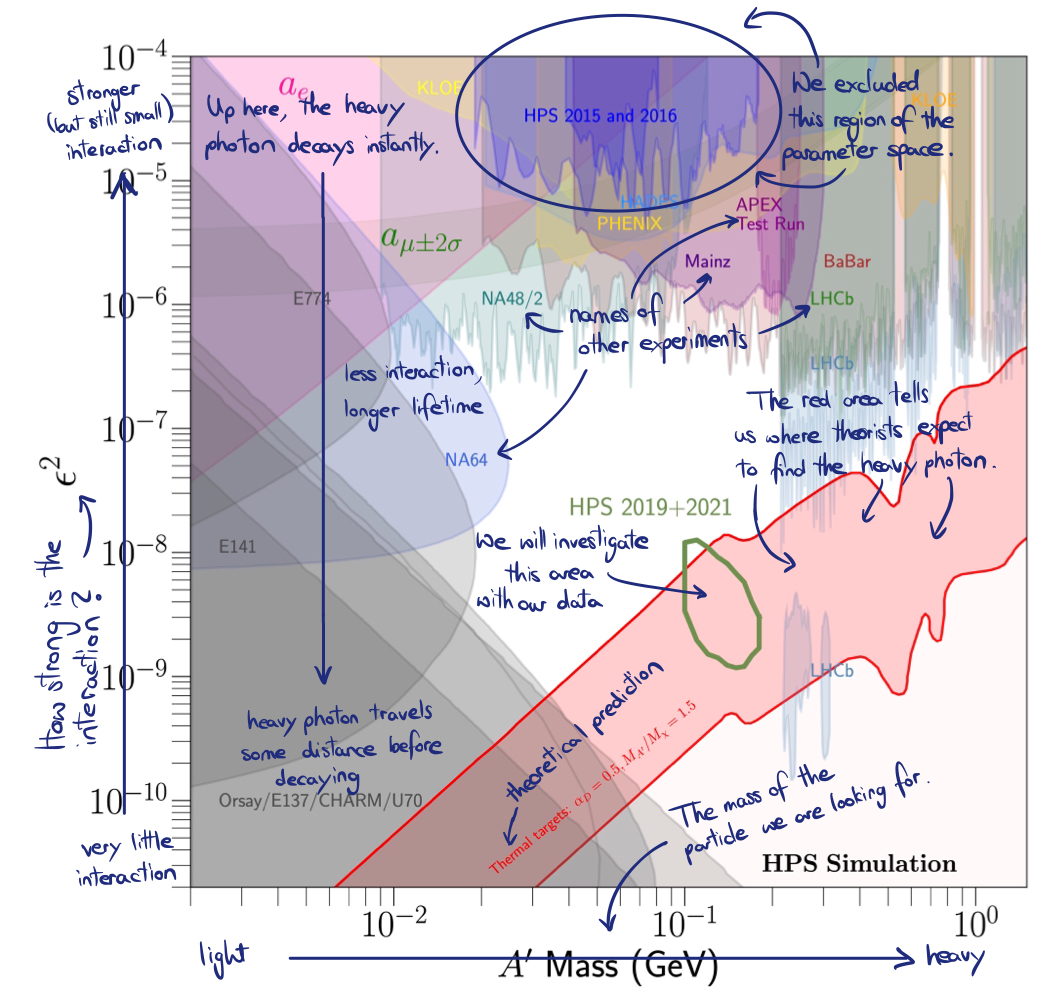
\includegraphics[width=\columnwidth]{figs/HPSreach.jpeg}
%			{\color{white}placeholder}\\
			So far, we haven't found the Heavy Photon. But that doesn't mean that we didn't learn anything in the process! Going through different combinations of masses and interaction strengths of the Heavy Photon with particles like electrons and positrons, we can exclude regions of the `parameter space' for which we don't see a signal in our data. This gives us a so-called `exclusion plot' that highlights masses and interaction strengths for which we didn't find the Heavy Photon. Many experiments besides HPS are searching for Heavy Photons. Hopefully, someone will find it soon!
		}


% \headerbox{box 9}{name=box9,column=1,below=box7,span=1}{
% \AtNextBibliography{\footnotesize}
% \setlength\bibitemsep{0pt}
% \printbibliography[heading=none]
% }

	\end{poster}
\end{document}